\chapter{Návrh platformy pro otevřené smlouvy}
\label{sec:kap6}

\section{Architektura}

Základem pro platformu pro otevřené smlouvy jsou tři nezávislé moduly. Konverzní modul, jednotné úložiště a webová aplikace. Každá zapojená veřejná instituce bude mít svůj konverzní modul. Jednotlivé konverzní moduly budou pracovat nad konkrétními relačními databázemi jednotlivých veřejných institucí a publikovat smlouvy jako Linked Open Data. Tato data pak budou ukládána v jednotném úložišti.

Základní otázkou, kterou si je třeba položit, je způsob shromažďování dat. První možností je směr centralizovaný, resp. každý konverzní modul publikovaná data pošle do jednotného úložiště. Druhým přístupem je decentralizace, kdy konverzní moduly vystaví data na internetu a registrují přístup k datům v datovém katalogu. Jednotné úložiště si poté taková data na základě katalogu obstarává samo. Výhoda první možnosti spočívá v snadnější udržitelnosti správy nad jednotlivými instancemi veřejných institucí. Subjekty mohou v určitém intervalu posílat převedené smlouvy do úložiště bez dalších nároků na správu. V druhém přístupu jsou naopak zvýšeny nároky na jednotlivé subjekty, které vypublikované smlouvy samy musejí  udržovat. Výhodou ale naopak je, že každý subjekt se stane lokálním úložištěm smluv, na které se lze odkazovat, např. na webových stránkách subjektu, vytvářet nad daty aplikace apod. První varianta je vhodná pro myšlenku centralizovaného registru, který pouze definuje podmínky, jak nahrávané smlouvy mají vypadat. Subjekty potom mají svobodu v tom, jak data převedou, pošlou, případně vypublikují. Druhá možnost naopak podporuje myšlenku, že každý subjekt zveřejňuje pouze své smlouvy a po vypublikování je umožní komukoli využít. Není proto překvapením, že myšlence otevřených a propojených dat vyhovuje více druhý přístup. 

K efektivnímu naplnění druhého přístupu je důležité, že součástí platformy bude konverzní modul, který převod za subjekty řeší a celý proces otevírání smluv pomůže zautomatizovat. Částečně tak vyřešíme nevýhodu druhého přístupu a část agendy otevírání smluv přebere platforma. Na konkrétním subjektu tak zbývá pouze udržovat v chodu databázi a server (typicky webový), kde konverzní modul poběží. 

Situaci můžeme dále zjednodušit tím, že subjekt zpřístupní svou databázi online. Konverzní modul tak bude moci pracovat nezávisle na subjektu a data pouze vzdáleně načítat. Narážíme zde ale na bezpečností limity. Databáze veřejných institucí bude typicky přístupná pouze v rámci privátní sítě. Řešením by mohlo být, že server, kde poběží konverzí modul, bude připojen do privátní sítě subjektu, druhou možností je např. klonování databáze smluv do veřejně přístupné databáze. Konkrétní řešení přístupu k databázi však necháme na konkrétních potřebách jednotlivých subjektů. Řekněme tedy, že konverzní modul platformy bude vyžadovat pouze připojení ke konkrétní databázi.

Základní pohled na platformu můžeme vidět na Obr. \ref{obr:logicalView}.

\begin{figure}[H]
\centerline{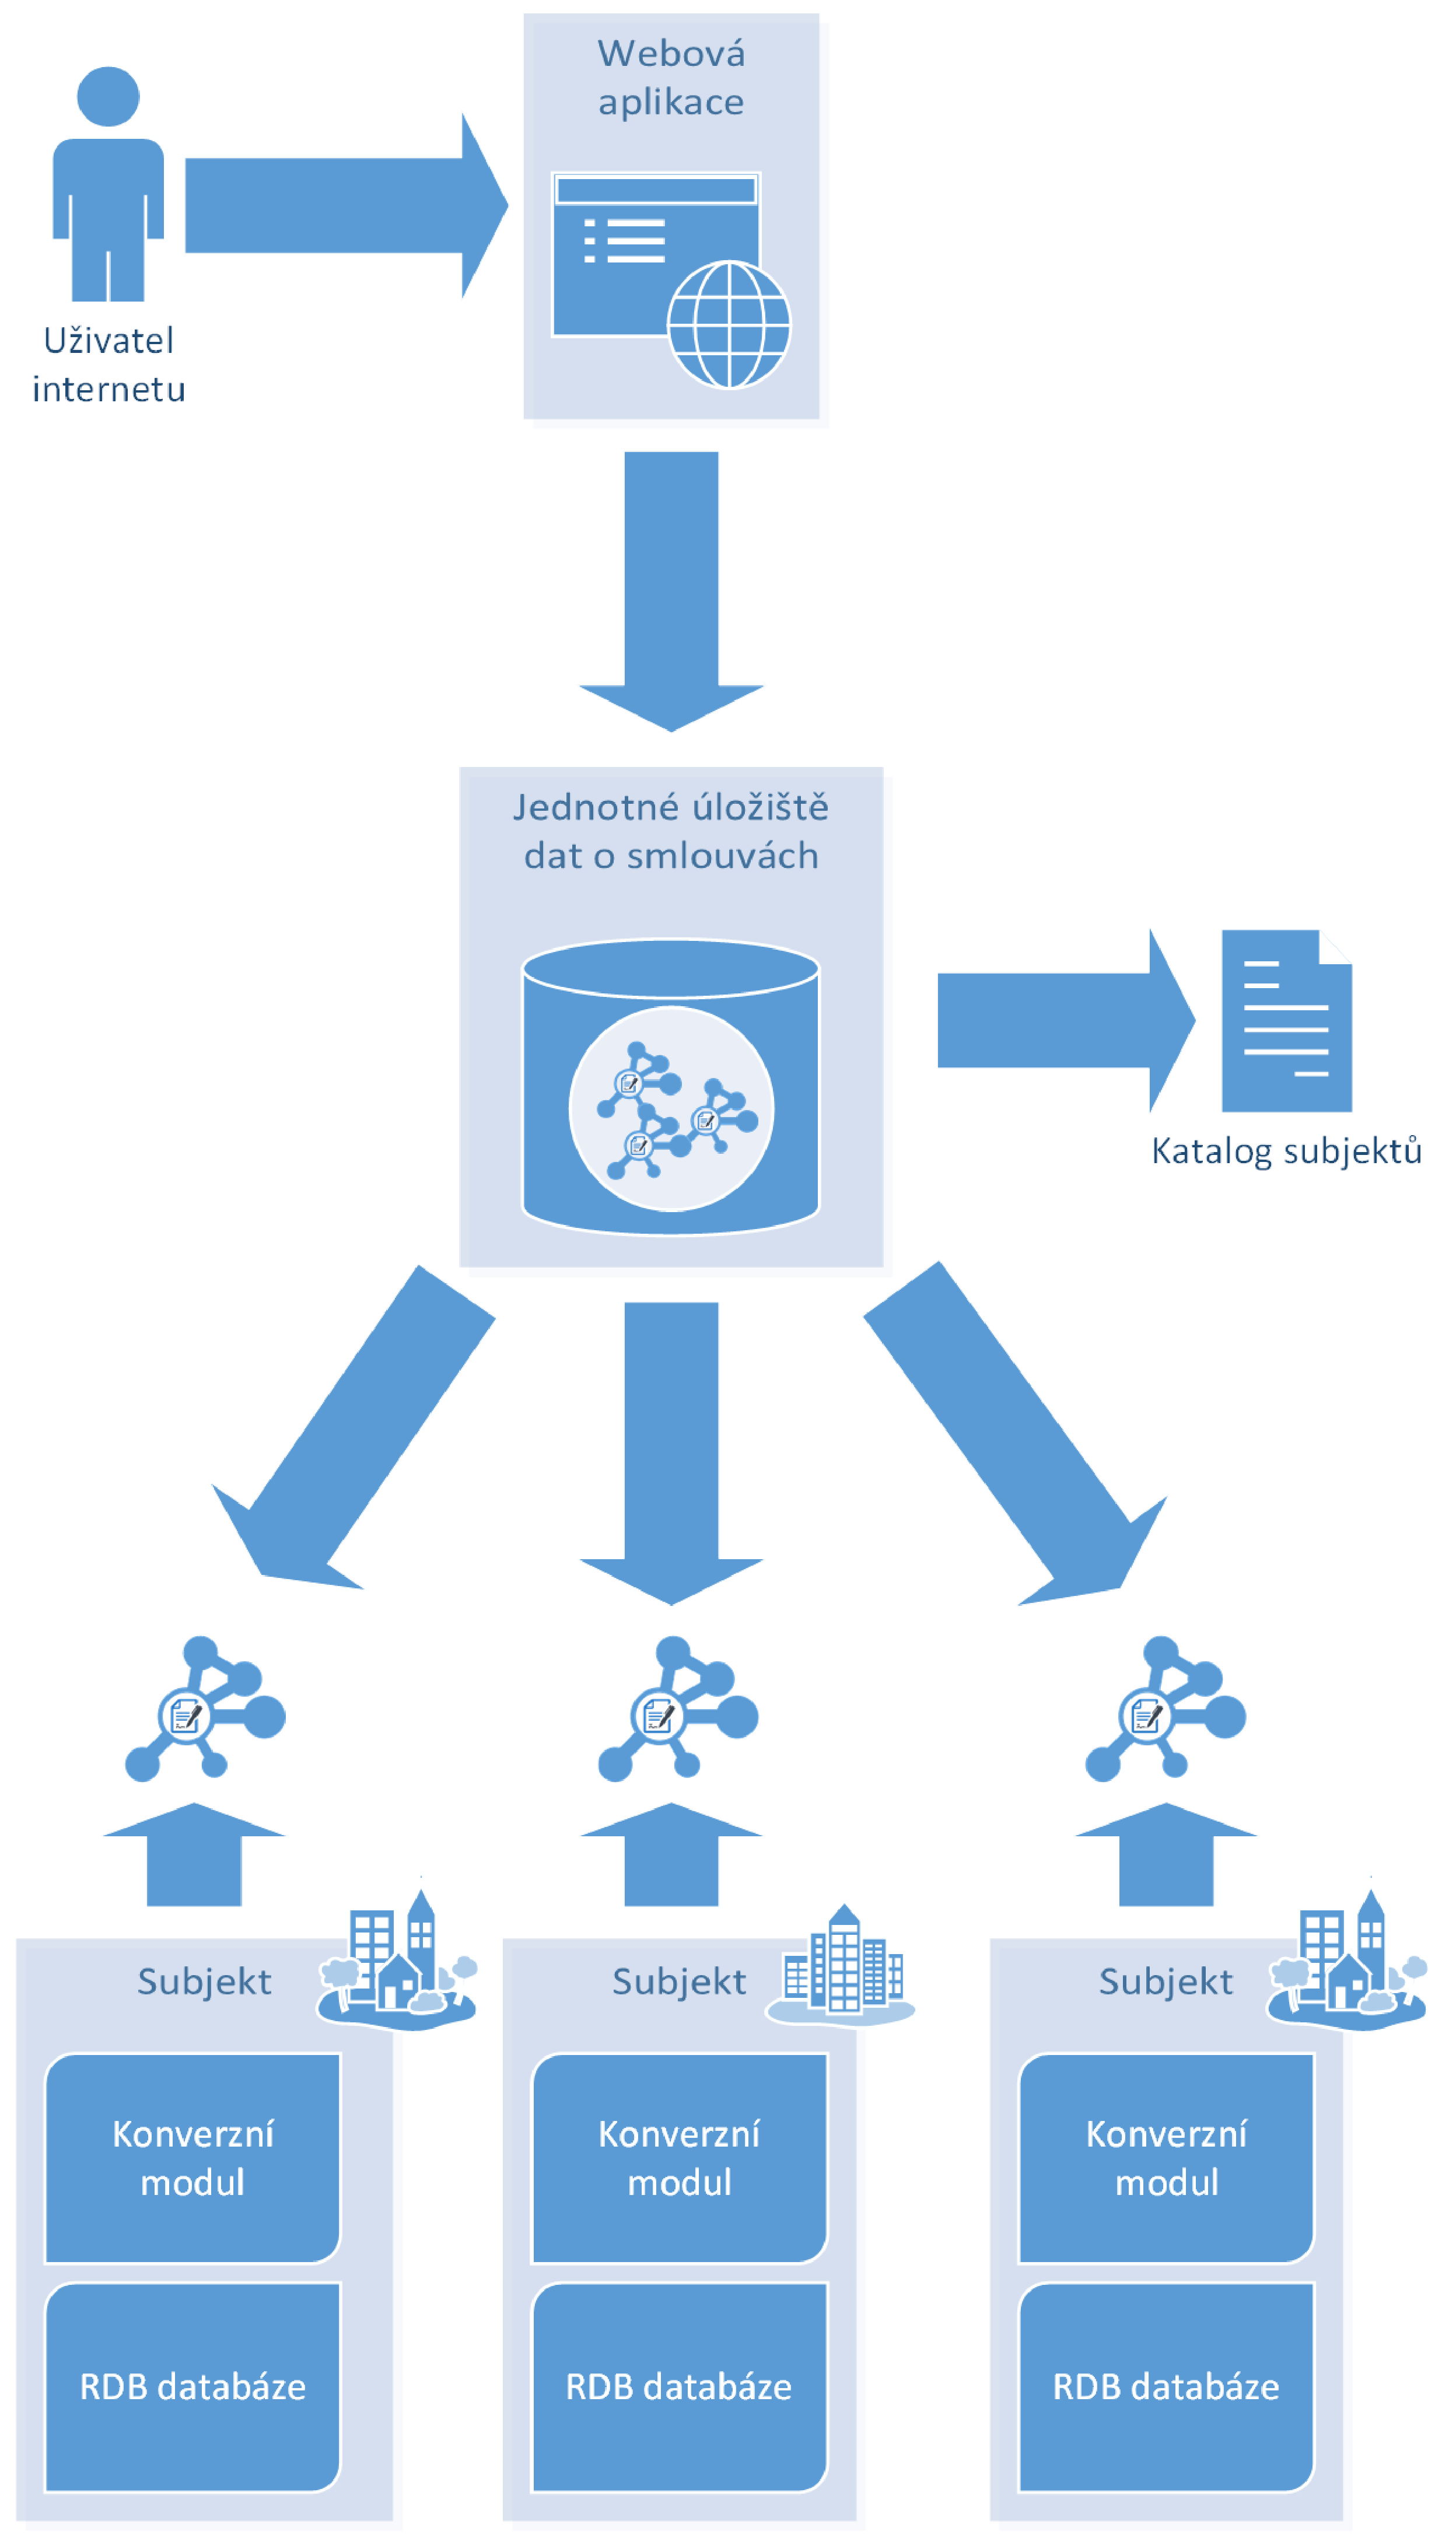
\includegraphics[width=135mm]{img/logicalView.eps}}
\caption{Základní pohled na platformu otevřených smluv (Logical view)}
\label{obr:logicalView}
\end{figure}

\begin{figure}[H]
\centerline{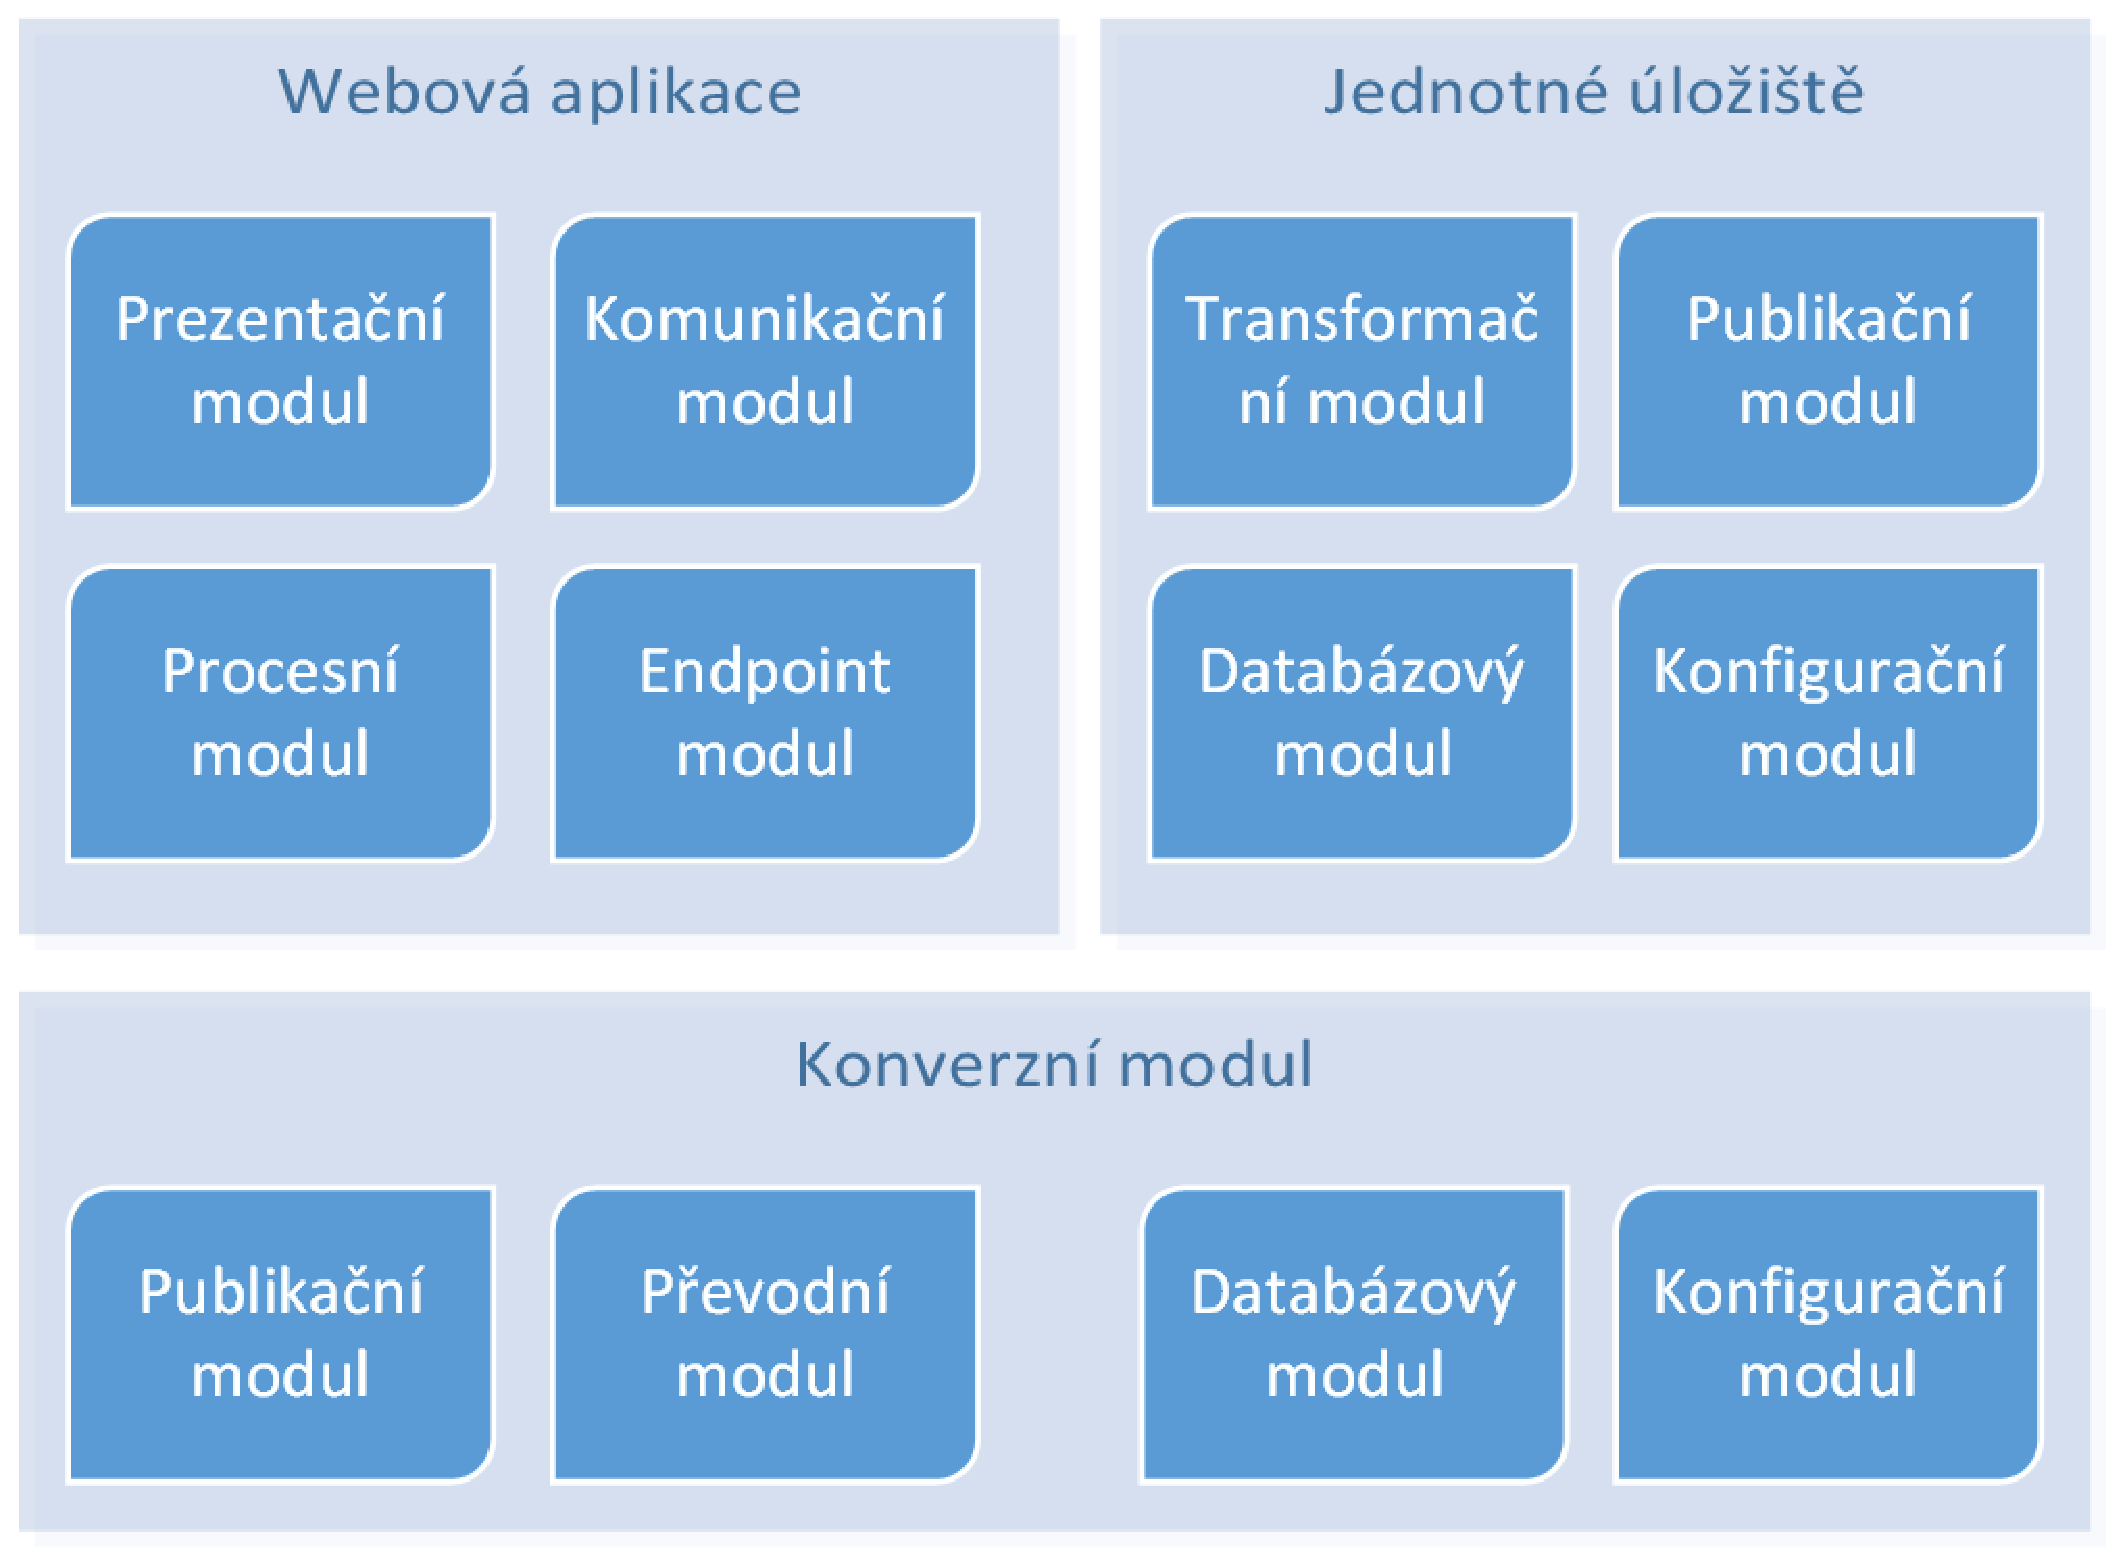
\includegraphics[width=\textwidth]{img/decompositionView.eps}}
\caption{Rozdělení platformy do modulů (Decomposition view)}
\label{obr:decompositionView}
\end{figure}

\section{Konverzní mechanismus}

Návrh konverzního mechanismu rozdělíme do čtyř modulů (viz Obr. \ref{obr:decompositionView}). V rámci databázového modulu bude docházet ke komunikaci mezi připojenou databází a zbytkem konverzního mechanismu. V konfiguračním modulu se očekává definování základních vlastností konverzního mechanismu, převážně potřebné vstupní údaje pro převodní modul.

\subsection*{Převodní modul}

Účelem tohoto modulu je převod relačních dat do RDF podoby. Nejjednodušším přístupem je manuální konverze, resp. ruční tvorba RDF výstupů. Tento přístup může být vhodný pro úzce specifické situace, avšak pro obecný přístup a možnost znovupoužití konverzního modulu vhodný není. Další možností je tvorba paralelní triplestore databáze. Relační data bychom v určitých intervalech převáděli z jedné do druhé. Tento přístup je výhodný, pokud chceme dosáhnout robustního řešení, budovat vlastní RDF úložiště, obohacovat data, přidávat další datasety apod. Klade však velké softwarové i hardwarové nároky na subjekt, vyžaduje netriviální údržbu a jedná se v podstatě o duplikovaná data z relační databáze. Poslední možností, kterou uvedeme, je tvorba wrapperu nad relační databází. Máme-li požadavek na RDF data, wrapper ho převede na ekvivalentní SQL dotaz do databáze a vrácená data převede zpět do odpovídající RDF podoby. Hlavní výhodou je, že takto uložená data jsou pouze v relační databázi a RDF data jsou tak vždy aktuální. Cílem je řešení s co nejmenší zátěží pro subjekt a s co nejlepším usnadněním znovupoužitelnosti. Ideálním řešením se tedy jeví tvorba wrapperu.

Požadovanou funkcionalitou wrapperu je namapování datového modelu relační databáze na datový standard pro otevřené smlouvy. Mezi jazyky sloužící k popsání konkrétního mapování patří např. jazyk R2RML\cite{R2RML}, nebo D2RQ\cite{D2RQ}. V rámci MFF UK vznikají projekty pracující nad R2RML (s potenciálem využití), jazyk je navíc doporučeným standardem konsorcia W3C. Zvolíme tedy jazyk R2RML\footnote{Principem jazyka R2RML je mapování tabulek pomocí tzv. \uv{triples map}. Jedná se o pravidlo v rámci kterého se definuje nad konkrétní tabulkou mapování subjektu a následně sada pravidel pro mapování dvojic predikát/objekt. Typicky pak subjekt reprezentuje konkrétní tabulku, predikáty jednotlivé sloupce a objekty uložené hodnoty.\cite{R2RML} }.

\subsection*{Publikační modul}

Převedená data můžeme publikovat třemi základními způsoby:

\begin{itemize}
\item Dump - veškerá data jsou zpřístupněna formou stažitelného souboru serializovaného v nějakém z RDF formátů
\item Dereferencovaná URI jednotlivých entit - každá entita je dostupná pod svým URI, typicky ve formě HTML stránky
\item API - v kontextu RDF se typicky jedná o webovou službu ve formě SPARQL endpointu umožňující libovolné dotazování nad daty.
\end{itemize}

Naší snahou je, aby vypublikovaná data mohly využívat i jiné aplikace, než pouze jednotné úložiště v rámci platformy. K tomu je ideální API. Zvolíme proto SPARQL endpoint.

Pro naplnění principů Linked Data ale potřebujeme vyřešit dereferencování URI entit. Nad SPARQL endpointem se dereference provede jednoduše tak, že každé HTTP URI odkazující na konkrétní entitu se převede na vhodný SPARQL dotaz vracející požadovaná data. 

Data budou publikována jak ve formě HTML stránky, tak v RDF formátech. Nutným základem bývá formát N-Triples a Turtle. Určíme podmínku, že pro dump je nutné umožnit i serializaci ve formátu JSON-LD z důvodu budoucí kompatibility s datovým standardem.

\subsection*{Anonymizace} 

Typickým problémem s publikací dat je, že mohou podléhat zákonu o ochraně osobních údajů\cite{z101}. Některá data je proto před zveřejněním nutné anonymizovat. Proces a řešení anonymizace není předmětem této práce. Řekněme, že platforma počítá s tím, že subjekt si anonymizaci údajů vyřeší na své straně.

\section{Jednotné úložiště}

Agendou jednotného úložiště bude sbírat data vypublikovaná jednotlivými subjekty. Zapojené subjekty budeme řešit formou datového katalogu, v kterém se budou nacházet odkazy na umístění požadovaných datasetů. Úložiště pak v definovaném intervalu stáhne datasety podle datového katalogu a uloží je do triplestore databáze.

Dekompozici do modulů je možné vidět na Obr. \ref{obr:decompositionView}. Databázový modul by měl obsluhovat komunikaci s triplestore databází. Konfiguračním modulem je míněno nastavení procesů jednotného úložiště včetně nastavení intervalu stahování datasetů.

\subsection*{Transformační modul}

V prvním kroku je třeba načíst jednotlivé datasety subjektů. Odkazy na konkrétní datasety budou reprezentované ve formě datového katalogu. Samotný katalog budeme zapisovat v RDF a serializovat do formátu Turtle. Využijeme k tomu ontologii Data Catalog Vocabulary. Příklad datového katalogu lze vidět v kódu \ref{lst:subject_catalog}.

V dalším kroku je třeba vyřešit otázku heterogenity dat. Platforma by principiálně měla umět přijímat RDF data nejen od subjektů zpracovaná konverzním modulem, ale i jakákoli jiná RDF data splňující datový standard a reflektující definovanou RDF ontologii. Jednotlivé entity by ale měly být identifikované podle vzoru z kapitoly~\nameref{sec:kap4}. To nám zaručí, že žádné dvě entity různých subjektů nebudou mít díky rozdílným doménám stejné URI. 

Díky tomu tak můžeme v rámci závěrečného kroku data slít dohromady a uložit do triplestore databáze.

\lstinputlisting[label=lst:subject_catalog, caption=Datový katalog pro jednotné úložiště, language=XML]{code/subject_catalog.ttl}

\subsection*{Publikační modul}

Úložiště by mělo data poskytovat jak k webovému prohlížení, tak skrze API k využití v aplikacích. Tento požadavek vyřešíme vystavením SPARQL endpointu. Typickou součástí publikace je také registrace datové sady v datovém katalogu.

\section{Datová síť}

Nad jednotným úložištěm může vznikat celá řada aplikací využívajících data o smlouvách. Díky propojení smluv se souvisejícími daty, tak můžeme kontext smluv rozšířit o další informace, resp. demonstrovat výhody principů Linked Data jako datové sítě.  

V rámci kapitoly \ref{sec:kap4} jsme definovali odkaz na veřejnou zakázku (pco:Contract) v rámci smlouvy, resp. predikát pco:publicContract ze smlouvy (třída cn:Contract) a odkaz na ekonomický subjekt (gr:BusinessEntity) pomocí predikátů owl:sameAs ze Smluvní strany a Vydavatele (třídy foaf:Organization a gr:BusinessEntity). Nyní si položme otázku, s jakými dalšími relevantními zdroji můžeme data na základě definovaných odkazů dále propojit.

Navrženou datovou síť propojených objektů můžeme vidět na Obr. \ref{obr:architectureLinks}. Z každého datasetu (v oválných blocích) vede hrana k vlastnímu objektu. Z nich pak vychází vybrané predikáty odkazující na entitu dalšího datasetu. 

Výchozím bodem je entita ekonomického subjektu (gr:BusinessEntity) uprostřed. Konkrétně se jedná o registrované organizace, jejichž data vychází z údajů na Profilu zadavatele, z ARESu a dalších zdrojů. Z této entity využijeme predikáty (s:address) k propojení s adresou (s:PostalAddress) z ARESu. Z adresy, pak získáme informaci o adresním místu (s:Place) z RUIANu pomocí predikátu ruianlink:adresni-misto.

Z entity ekonomického subjektu můžeme získat informaci o odpovídajícím objektu reprezentovaném v rámci orgánů veřejné moci díky zpětnému odkazu reprezentovanému predikátem ovm:business-entity. 

Propojení dosáhneme také mezi ekonomickým subjektem a veřejnou zakázkou (pco:Contract). Z veřejné zakázky využijeme odkazu na zadavatele, resp. predikátu (pco:contractAuthority). Díky tomu můžeme zjistit údaje o veřejných zakázkách jednotlivých ekonomických subjektů, kde vystupují v roli zadavatele.

Vydavatel smluv (foaf:Organization) je často veřejná instituce mající svoji stránku na DBpedii. Nedisponujeme však přímým odkazem na konkrétní reprezentaci vydavatele v DBpedii. Můžeme ale položit SPARQL dotaz, zdali v DBpedii existuje instituce s daným konkrétním jménem (porovnáním predikátů gr:legalName vydavatele a rdfs:label z DBpedie). Nejedná se tedy o přímé propojení, ale o další možnost, jak kontext smluv obohatit o další informace.

\begin{figure}[H]
\centerline{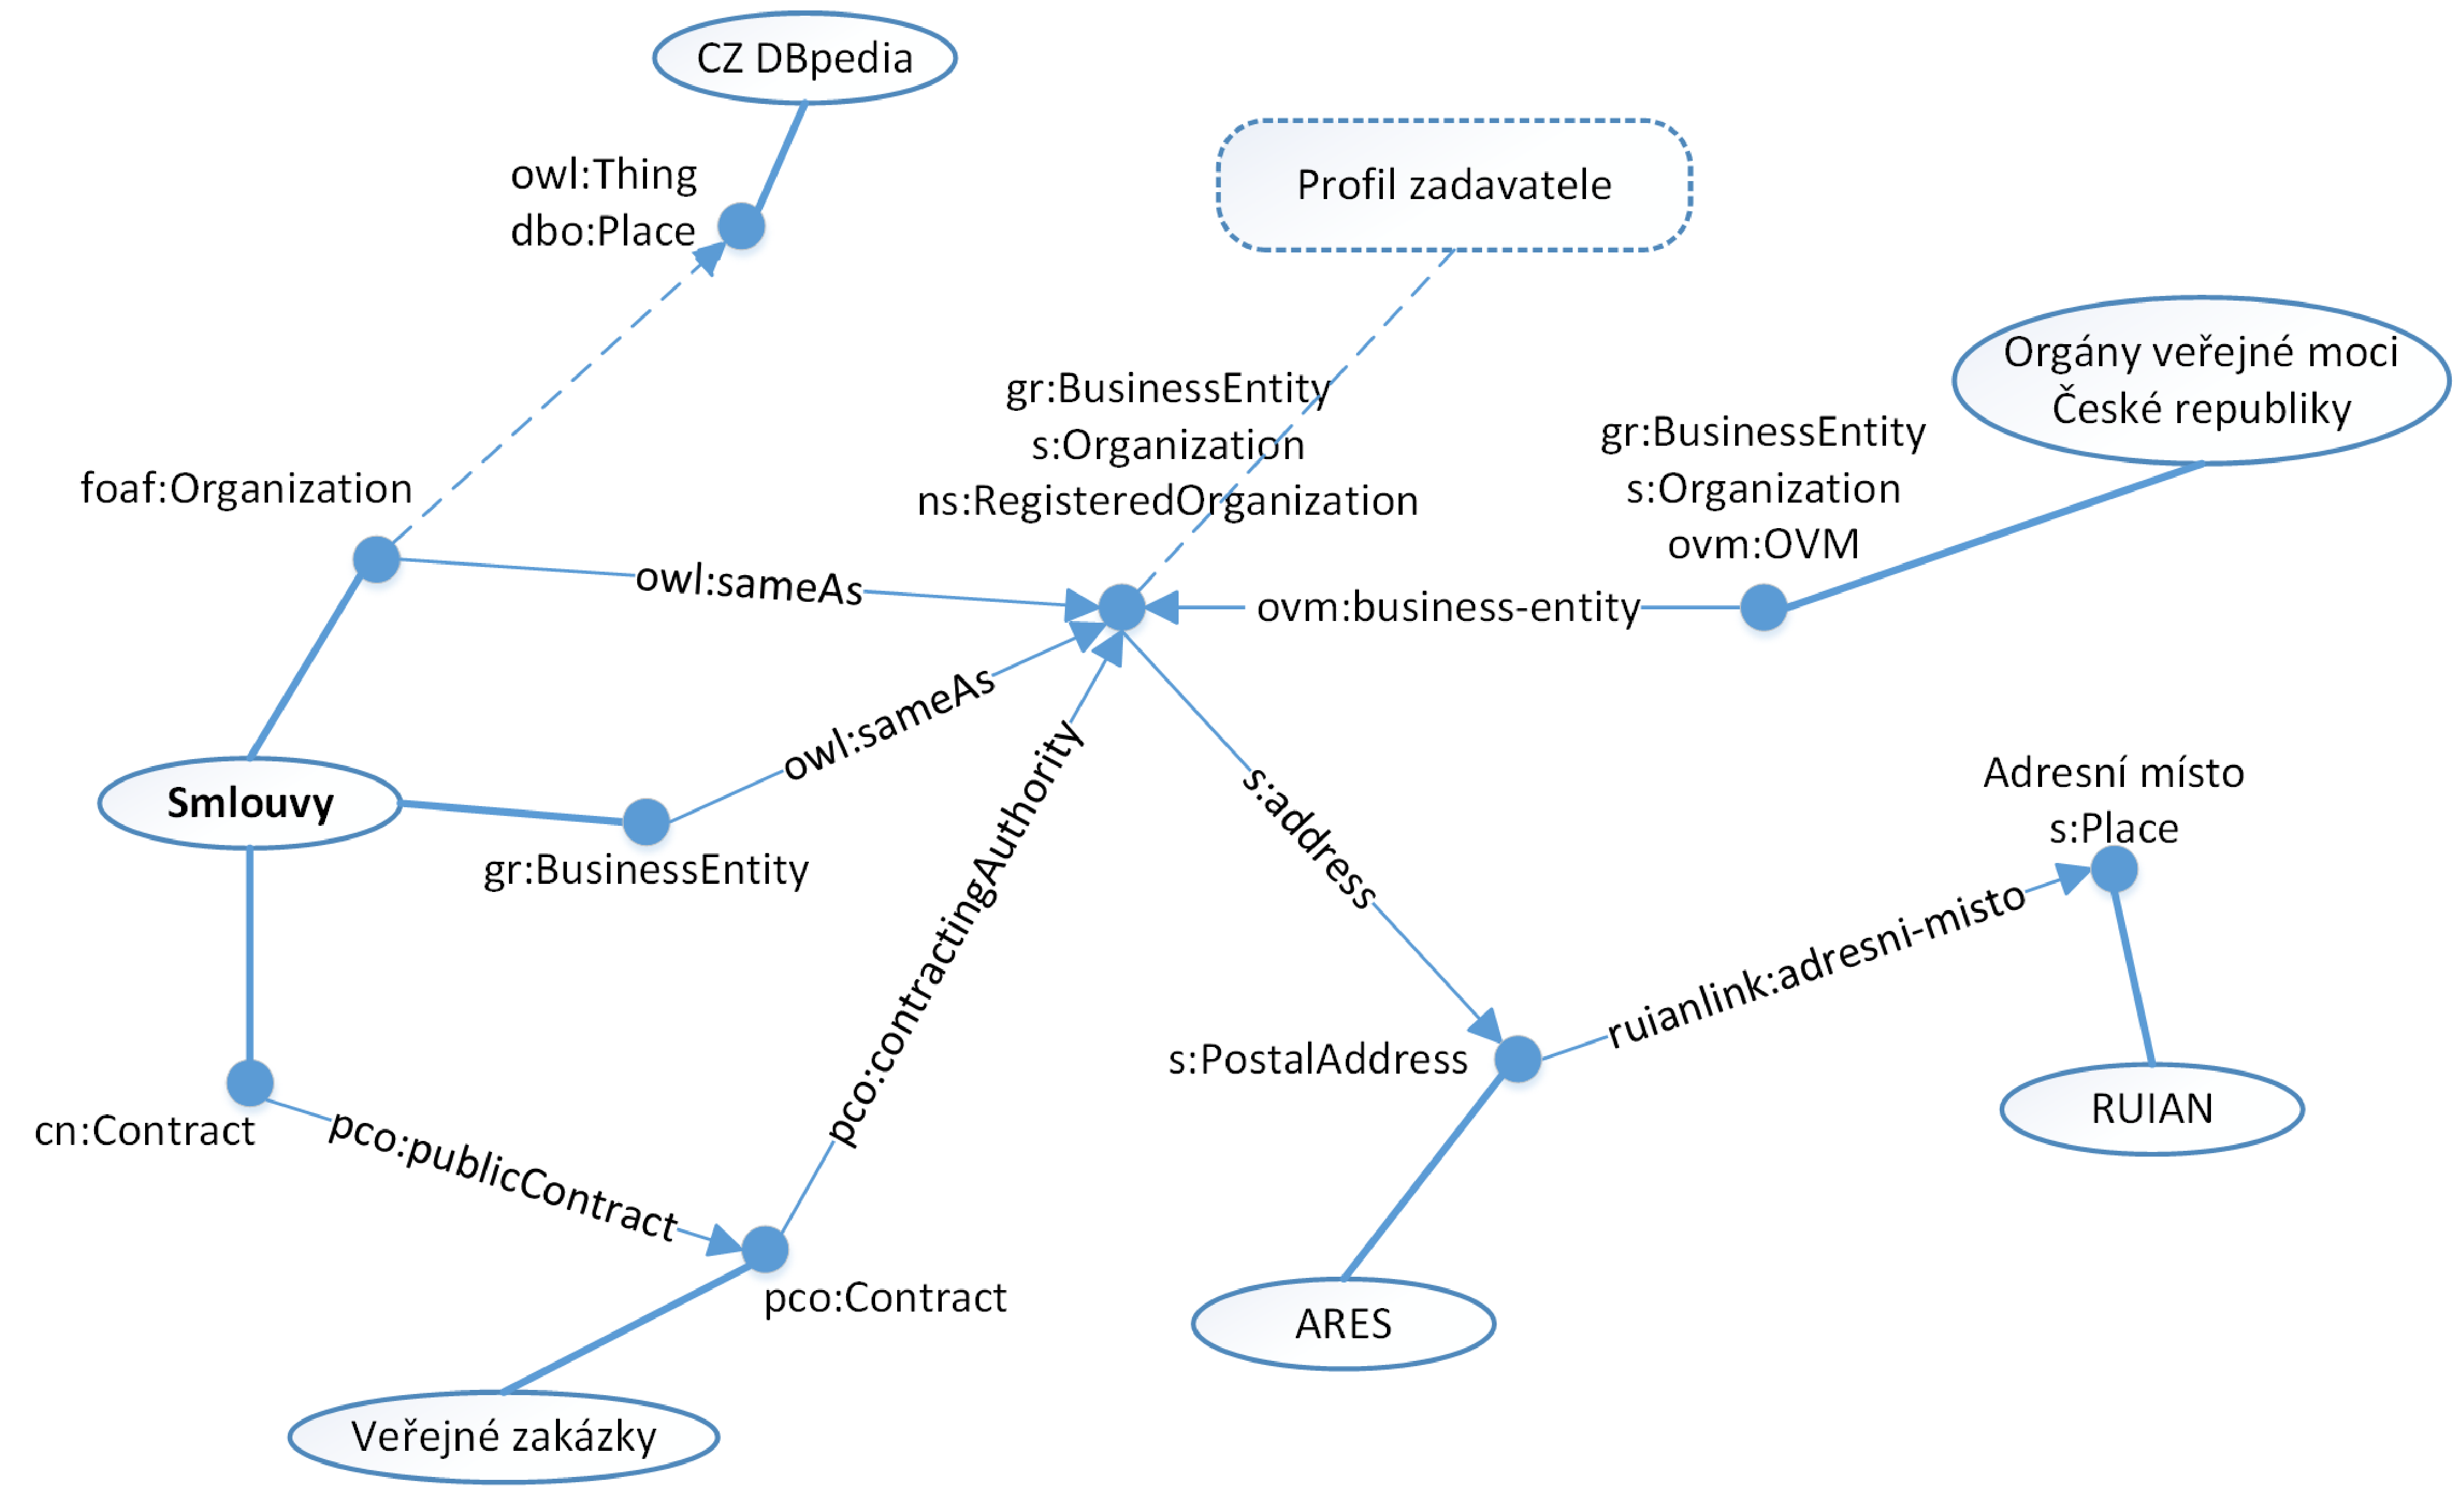
\includegraphics[width=\textwidth]{img/architectureLinks.eps}}
\caption{Datová síť}
\label{obr:architectureLinks}
\end{figure}

\section{Webová aplikace}

Úkolem webové aplikace je nad jednotným úložištěm zpřístupnit údaje o smlouvách k prohlížení koncovým uživatelům. Řešení rozdělíme do čtyř modulů (viz Obr. \ref{obr:decompositionView}).

\subsection*{Endpoint modul}

V rámci tohoto modulu definujeme napojení na požadované zdroje dat v podobě SPARQL endpointů.

\subsection*{Procesní modul}

Úkolem tohoto modulu je načíst požadované údaje o smlouvách a přiřadit k nim údaje z rozšířeného kontextu navrženého v minulé kapitole. Cílem je tedy získat a sjednotit informace z několika zdrojů dat.\footnote{Ukázka skici obohaceného kontextu smluvních údajů viz Obr. \ref{obr:linkedDataAdv}} Existuje několik přístupů, jak se nad požadovanými daty dotazovat\footnote{Předpokládejme, že aplikace bude obsahovat serverovou část.} - z klientské části aplikace, nebo ze serverové. Z důvodu dalšího zpracování dat se jeví vhodnější serverové dotazování. Samotné dotazy můžeme pokládat také různými způsoby. Jednou z možností je distribuované dotazování, kdy se v rámci jednoho dotazu můžeme odkazovat na více zdrojů. Další možností je se nad každým zdrojem dotazovat zvlášť, resp. sadou dotazů. V souladu s principy Linked Data zvolíme sadu dotazů nad jednotlivými SPARQL endpointy. Výhodou je, že problém jednoho zdroje by neměl ovlivnit výsledky z ostatních zdrojů. 

Nad SPARQL endpointy můžeme získávat data buď ve formě RDF (příkaz Construct), nebo v tabulkové formě (příkaz Select). Účelem je zobrazení dat uživateli často právě ve formě tabulek. Volba příkazu Select je tedy lepší volbou.

\subsection*{Komunikační modul}

Agendou komunikačního modulu je výměna dat mezi procesním a prezentačním modulem. Modul zpracuje požadavky z prezentačního modulu a volá konkrétní funkce procesního modulu. Výsledná data pak pošle prezentačnímu modulu k zobrazení. Rozhraní pro přenos by mělo být ve standardizovaném datovém formátu\footnote{Typicky v XML, nebo JSON}.

\subsection*{Prezentační modul}

Účelem tohoto modulu je zobrazování dat uživateli. Výchozím bodem je nabídnout přehledné informace o otevřených smlouvách. Úvodní obrazovku bude tvořit pohled vyznačující subjekty otevírající smlouvy (ideálně na mapovém podkladu) a následně souhrnný seznam všech smluv. Z informací o subjektech půjde přejít na detail vybraného subjektu. Dále z každé položky seznamu půjde přejít jak do detailu konkrétní smlouvy, tak do detailu jejího vydavatele (subjektu). Detail smlouvy zobrazí podrobné informace o zvolené smlouvě, včetně jejích verzí, smluvních stran, příloh, dodatků a milníků. Ze subjektů a smluvních stran majících vyplněný IČ půjde přejít na seznam veřejných zakázek, ve kterých subjekt vystupuje. Detail vydavatele nabídne podrobnější informace o zvoleném publikujícím subjektu. Součástí detailu vydavatele bude také seznam jeho smluv. Z tohoto seznamu půjde také přejít na detaily jednotlivých smluv.

\begin{figure}[H]
\centerline{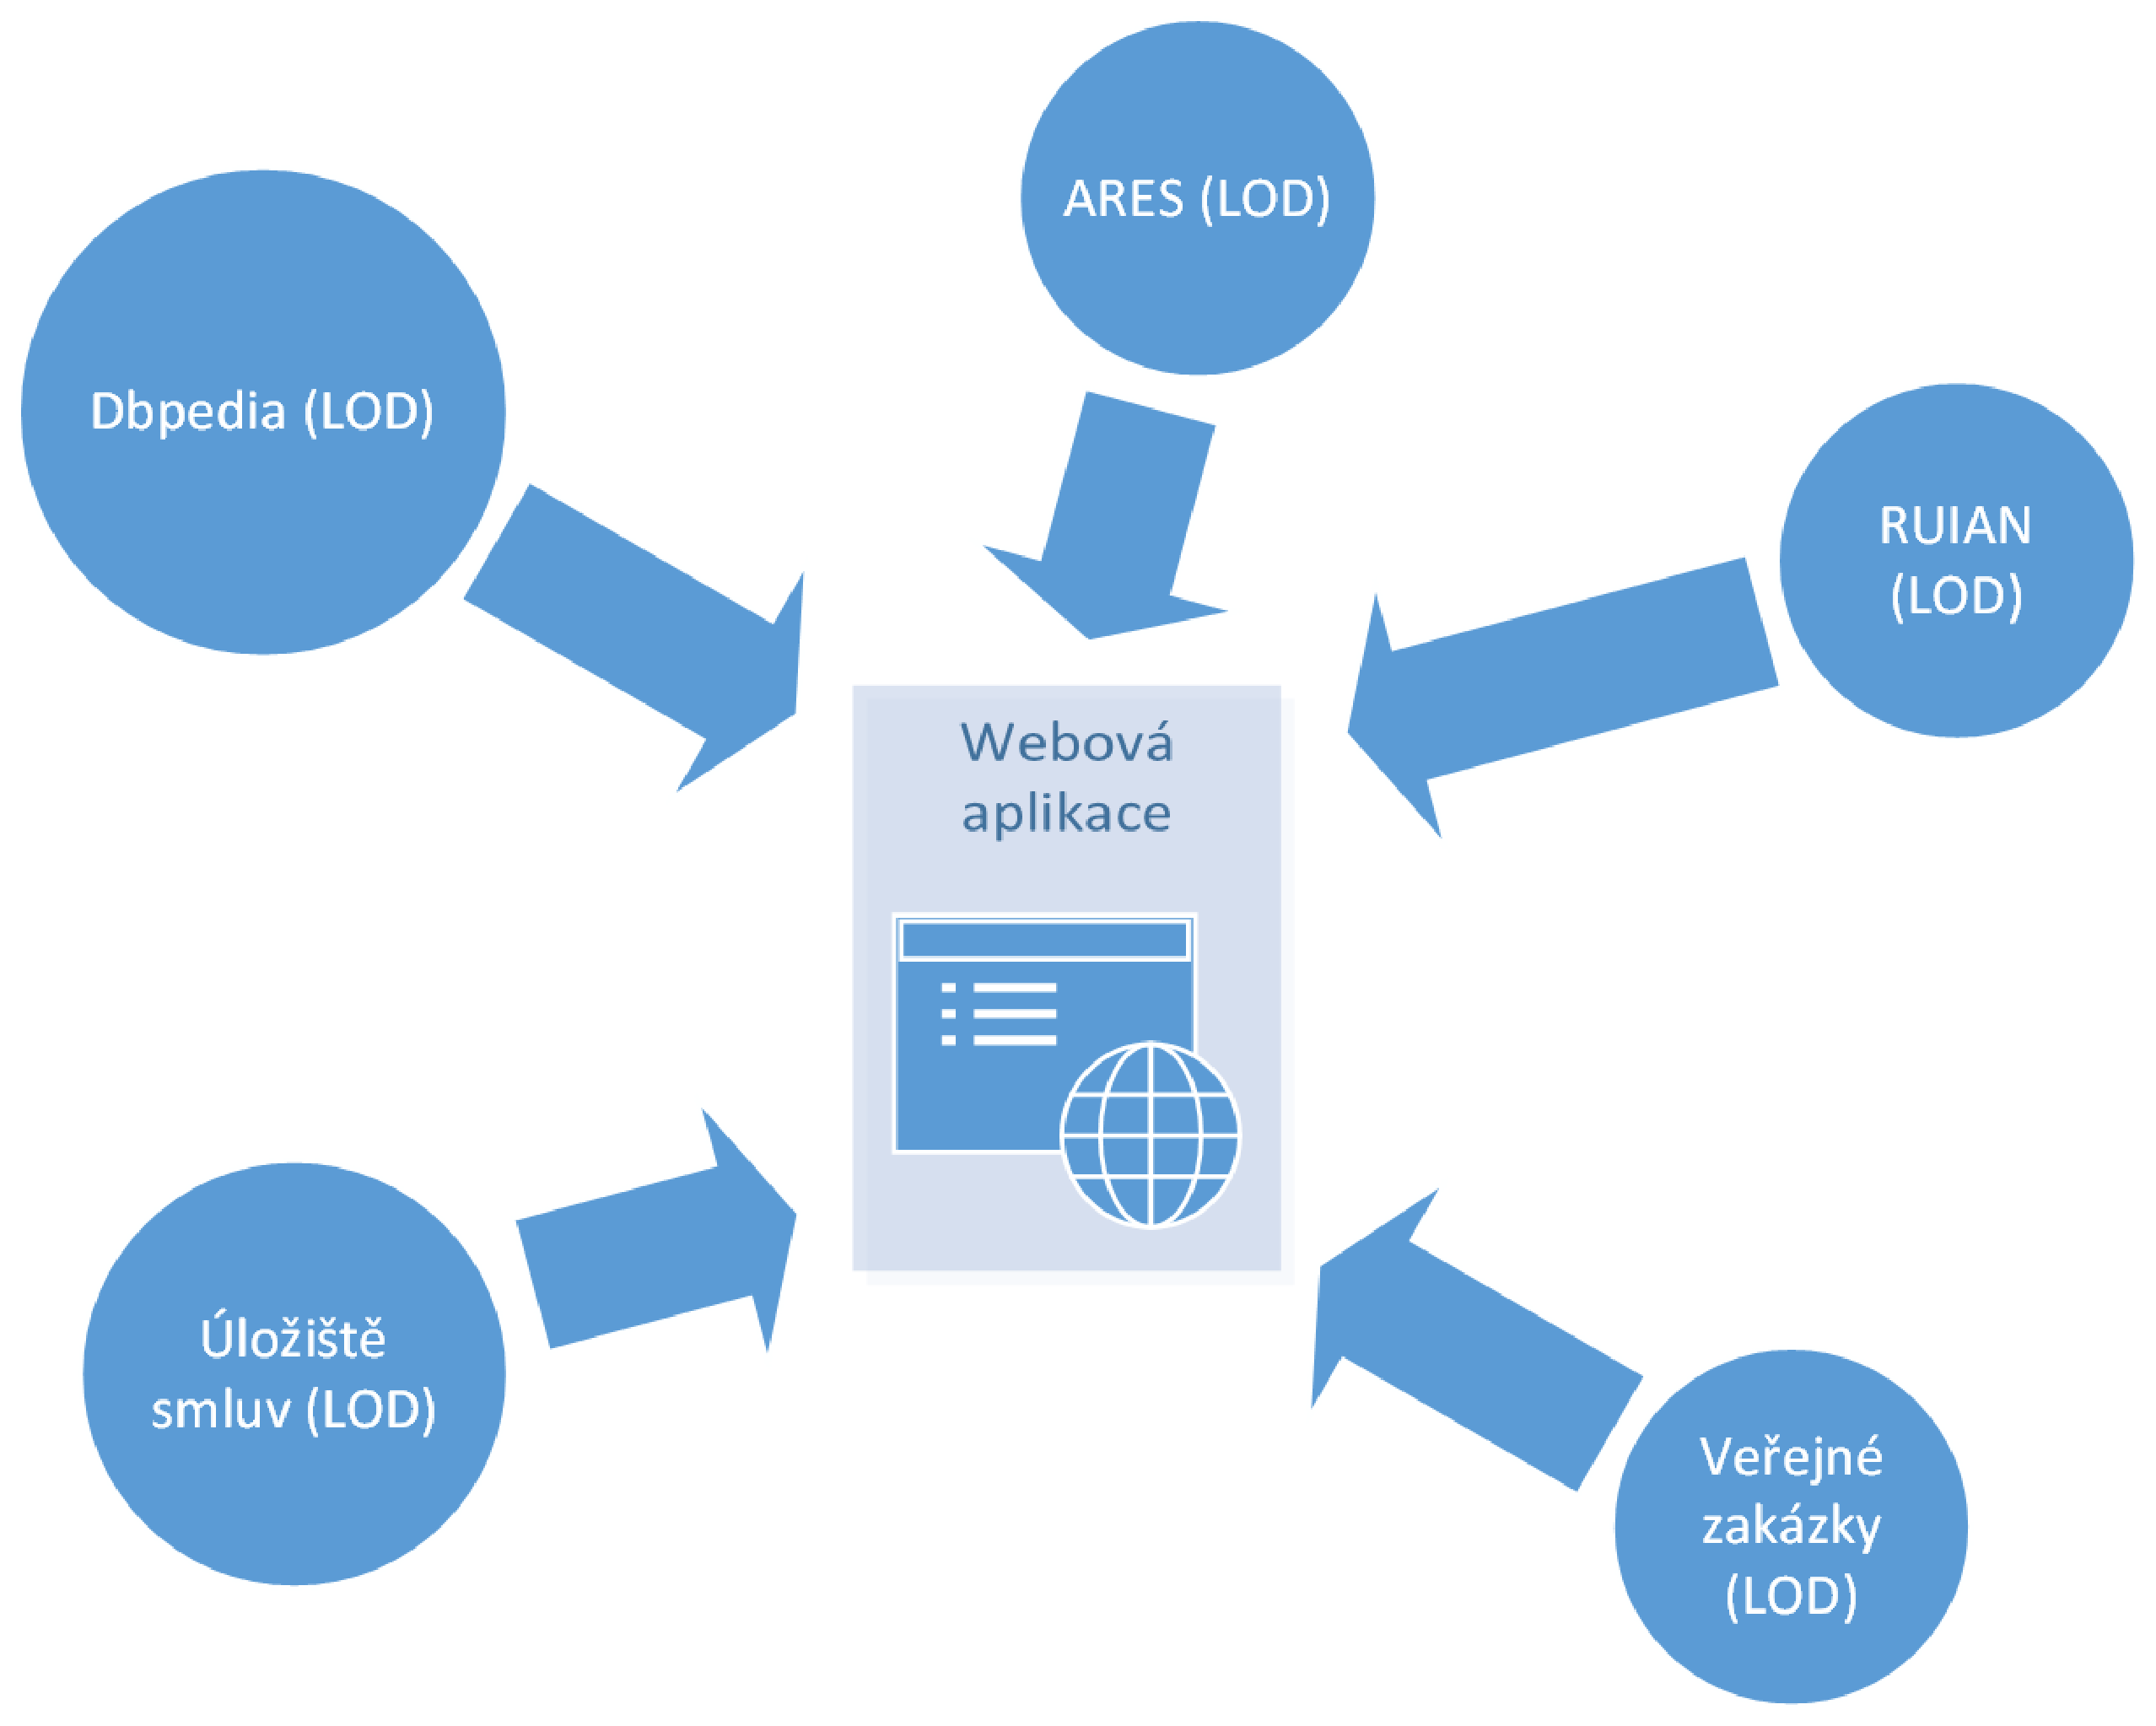
\includegraphics[width=120mm]{img/linkedDataAdv.eps}}
\caption{Obohacený kontext smluv díky propojeným datům}
\label{obr:linkedDataAdv}
\end{figure}